\section{PatternObject}\label{patternObject}

Accepts NoteProcessors: yes

Pattern Object

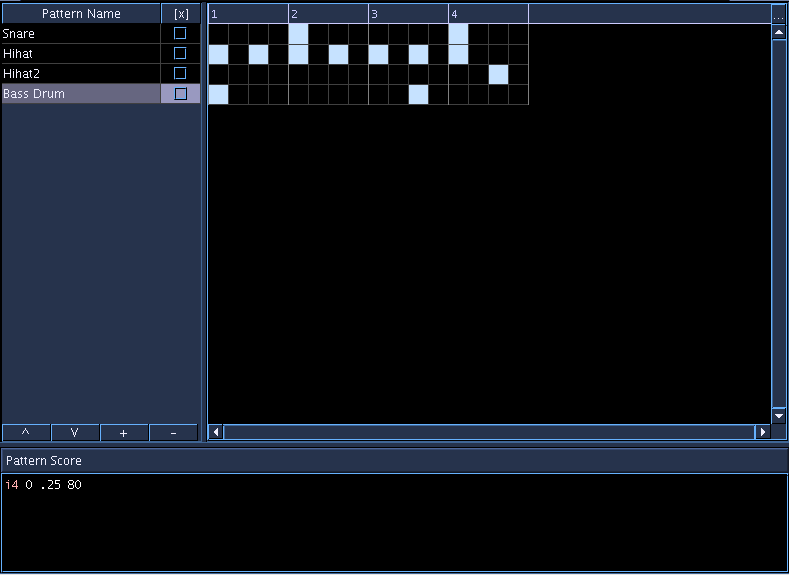
\includegraphics{images/patternObject1.png}

The PatternObject is pattern-based score editor, based on the author's
previous project "Patterns". It is a flexible pattern-oriented score
editor, useful for musical ideas which are pattern based, such as drum
parts or minimalist-style musical ideas.

For the general workflow of using the PatternObject, users will liked
likely want to:

\begin{enumerate}
\def\labelenumi{\arabic{enumi}.}
\item
  Setup the PatternObject Properties (number of beats and subdivisions)
\item
  Add Patterns, giving each pattern a name to help identify what the
  pattern is for
\item
  Edit each Pattern's score
\item
  Visually edit the PatternObject score
\end{enumerate}

The PatternObject's Time Properties can be modified by clicking on the
button in the upper-right corner of the editor. Clicking the button will
hide or show the properties panel on the right, as shown below:
PatternObject - Properties PatternObject - Properties

\begin{quote}
\textbf{Note}

Editing the time values will clear out any pattern triggers that the
user has entered. It is recommended that one first decide the pattern
time properties before working with the PatternObject.
\end{quote}

To add Patterns to the PatternObject, use the "+" button on the bottom
of the left hand section. Double-clicking the name of the pattern name
will allow editing of the name, and clicking on the {[}x{]} box will
allow for muting the Pattern. Clicking on the Pattern in the table will
also bring up it's score in the area below.

The Pattern's score is standard Csound SCO text, with the same features
supported as by the GenericScore SoundObject. Each score should be
started from time zero. The Pattern's score should be set such that its
score's total duration fits within the time of the subDivision. For
example, if the properties set for the PatternObject's time values are 4
beats and 4 subdivisions, each beat is 1.0 in duration (corresponds to
p3 value of a note) and thus a single subdivision in this case would be
equivalent to .25. Scores shorter or longer than the subdivision length
are allowed, but one should be aware that the resultant score may or may
not longer than what is visually represented on the PatternObject score.

The PatternObject score is visually edited by click on squares which
correspond to subdivisions of the beat. For example, if a Pattern's
score is .25 in total duration, and the time value of the PatternObject
is set to 4 and 4, then clicking a square would be to insert a 16th note
in a score.

To add to the PatternObject score, simply click on the square where one
wishes to have a Pattern triggered. To remove, simply click on a
selected square. The user can also click and drag to add or remove
mutliple triggers.

\begin{itemize}
\item
  Users may be surprised at the generated score if time behavior is not
  set to None(while others may prefer to use Scale, which is the
  default). Please be mindful of this, especially when using
  PatternObjects and the SoundObject library, where the default for
  creating instances of SoundObjects is to have Time Behavior of Scale
  on the Instance SoundObject.
\item
  When the PatternObject is used with a Scale time behavior, you may not
  get the results you think you will get if the pattern is not filled in
  in the last subdivision of the beat. When blue goes to generate a
  score for a soundObject, with a scale time behavior, the score is
  first generated, then scaled to the duration of the soundObject. So,
  if you're pattern has empty subdivisions and you're expecting there to
  be a space at the end of your pattern, when you go to generate the
  CSD, the space won't be there.

  To get around this, you may want to use a time behavior of None, or
  you may want put in a "ghost note" in a Pattern layer, using a note
  like:

\begin{verbatim}
i 10000 0 .25
    
\end{verbatim}

  Where 10000 is not an instrument in use in your project. Then you can
  put in a trigger for this pattern in the last subdivision. What will
  happen is that blue will process the score with this note's time and
  thus will generate with this out to the CSD, but Csound will ignore
  the note.

  When the PatternObject is set to use a time behavior of Repeat, the
  same situation can occur as when using Scale if a Repeat Point is not
  set, as the default for Repeat when no repeat point is set is to take
  the generated score and repeat it after the duration of the last note.
  To prevent this, either use the ghost note technique above or set a
  repeat point.
\end{itemize}
